Particle physics is the branch of physics that seeks out the origins of the universe by probing and searching for new interactions at the highest energies. 
The field started as studies in electromagnetism, radiation, and further developed with the discovery of the electron.
What followed was more experiments to search for new particles, new models to describe the results, and new search techniques which demanded more data.
The balance in resources for an experiment bottlenecks how much data can be taken, so steps need to be taken to identify interesting interactions and optimize the storage and processing of this data.
This thesis investigates software performance optimization of the ATLAS experiment at CERN. 
Specifically, ways to modernize and optimize areas of the software framework, Athena, to improve input/output (I/O) during derivation production and create new tests that catch when specific core I/O functionality is broken.

\section{LHC and The ATLAS Detector}

\begin{figure}[h]
    \centering
    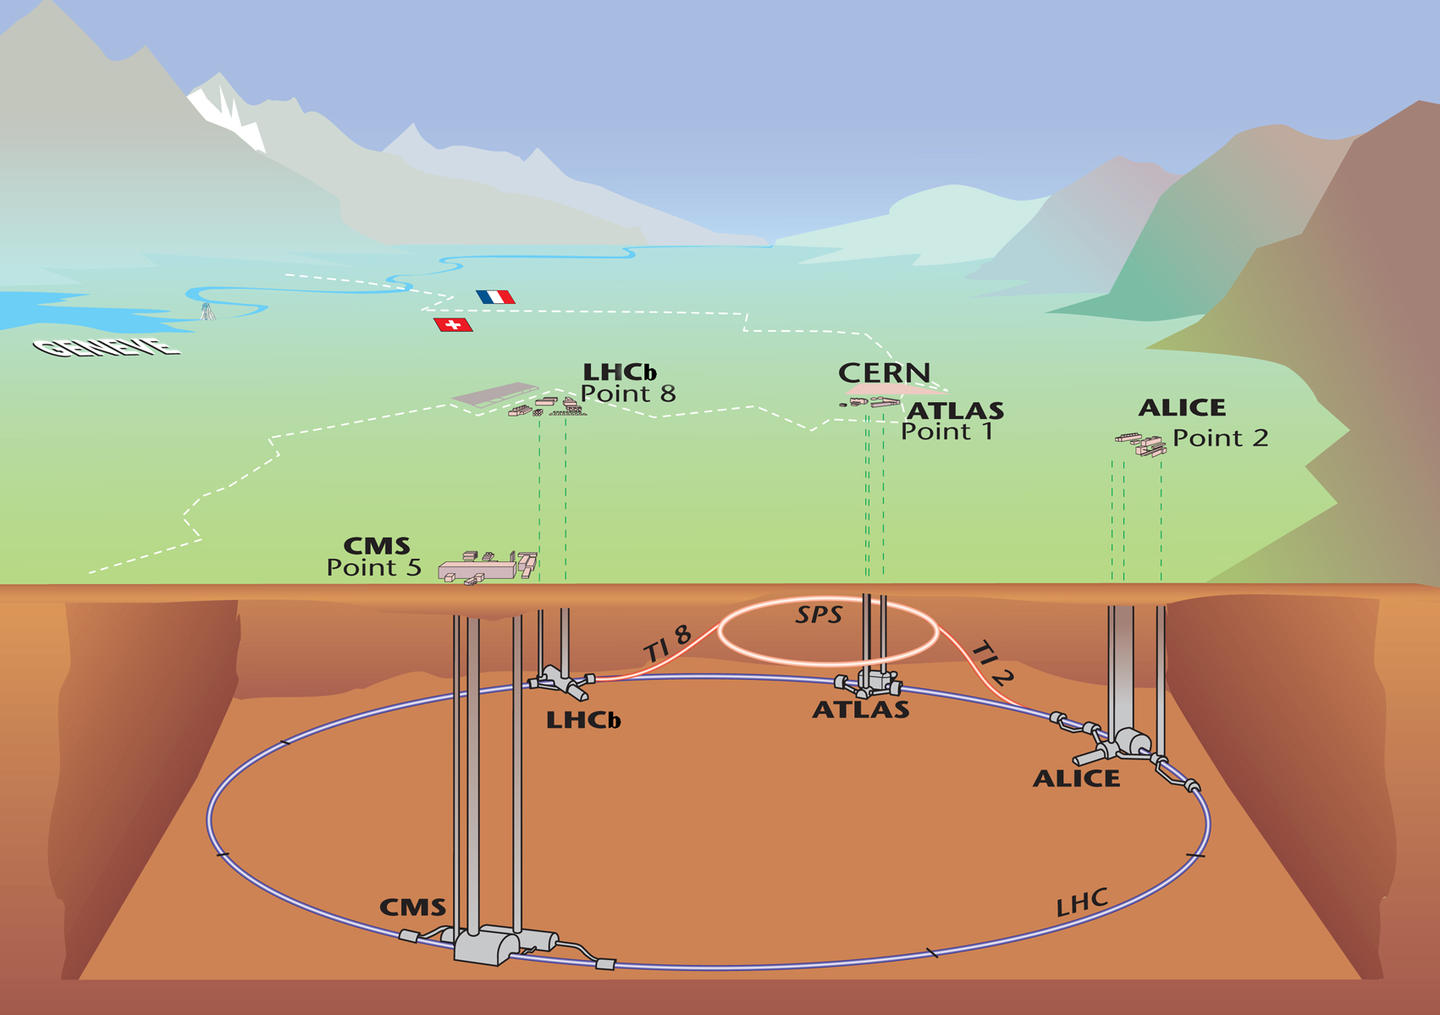
\includegraphics[width=.8\textwidth]{content/img/LHC illustration.jpg}
    \caption{Illustration of the LHC experiment sites on the France-Switzerland border. \cite{LHC_Illustration}}
    \label{fig:intro_LHC_sites}
\end{figure}

The LHC, shown in Figure \ref{fig:intro_LHC_sites},  is a 26.7-kilometer ring that crosses between the France-Switzerland border at a depth between 50 and 175 meters underground.\cite{LHC_faq_guide}
The ATLAS experiment, shown in Figure \ref{fig:intro_ATLAS_detector}, is the largest LHC general purpose detector, and the largest detector ever made for particle collision experiments. 
It's 46 meters long, 25 meters high and 25 meters wide.\cite{ATLAS_Fact_Sheet}
The ATLAS detector is comprised of three main sections, the inner detector, calorimeters and the muon detector system. 


\begin{figure}[h]
    \centering
    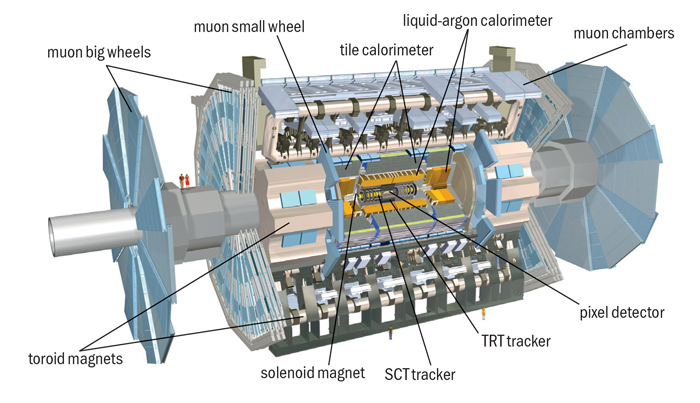
\includegraphics[width=.8\textwidth]{content/img/ATLAS_Detector.jpg}
    \caption{Overview of the ATLAS detectors main components. \cite{ATLAS_Illustration}}
    \label{fig:intro_ATLAS_detector}
\end{figure}


The inner detector measures the direction, momentum and charge of electrically charged particles.
It's main function is to measure the track of the charged particles without destroying the particle itself.
The first point of contact for ATLAS is the pixel detector. 
It has over 92 million pixels and is radiation hard to aid in particle track and vertex reconstruction.\cite{Hugging2006}
When charged particles pass through a pixel sensor ionizes silicon which produces an electron-hole pair, and this generates an electric current that can be measured. \cite{Giangiacomi:2684079}
Surrounding the pixel detector is the semiconductor tracker, which uses 4,088 modules of 6 million implanted silicon readout strips.
The semiconductor tracker helps measure the path particles take, called tracks, with precision up to $25\mu m$. 
The final layer of the inner detector is the transition radiation tracker (TRT). 
The TRT is made of a collection of tubes made with many layers of different materials with varying indices of refraction.  
Particles with relativistic velocities have higher Lorentz $\gamma$-factors, see Eq. \eqref{lorentzGamma}, the TRT uses varying materials to discriminate between heavier particles (with low $\gamma$ and radiate less) and lighter particles (higher $\gamma$ and radiate more). \cite{Mindur:2139567}
\begin{equation}\label{lorentzGamma}
    \gamma = \frac{1}{\sqrt{1 - \frac{v^2}{c^2}}}
\end{equation}

There are two main calorimeters for ATLAS, the Liquid Argon (LAr) calorimeter and the Tile Hadronic calorimeter.
The LAr calorimeter surrounds the inner detector and measures the energy deposits of electrons, photons and hadrons (quark bound states, such as baryons $qqq$ and mesons $q\bar{q}$). 
It layers various metals to intercept the incoming particles to produce a shower of lower energy particles. 
The lower energy particles then ionize the liquid argon that fill the barrier in between the metal layers to produce a current that can be read out.
The Tile calorimeter surrounds the LAr calorimeter and is the largest part of the ATLAS detector weighing in around 2900 tons. 
Particles then traverse through the layers of steel and plastic scintillating tiles. 
When a particle hits the steel, a new shower of particles is generated and the plastic scintillators will produce photons with a measurable current.

\section{ATLAS Trigger and Data Acquisition}

The LHC produces $pp$-collisions at a rate of 40 MHz, each collision is an ``event". 
% What is the ATLAS Trigger System
The ATLAS Trigger system is what's responsible for quickly deciding what events are interesting for physics analysis.
The Trigger system is divided into the first- and second-level triggers and when a particle activates a trigger, the trigger makes a decision to tell the Data Acquistion System (DAQ) to save the data produced by the detector. 
The first-level trigger is a hardware trigger that decides within $2.5 \mu s$ after the event occurs if it's a good event to put into a storage buffer for the second-level trigger.
The second-level trigger is a software trigger that decides within $200 \mu s$ and uses around 40,000 CPU-cores and analyses the event to decide if it is worth keeping. 
The second-level trigger selects about 1000 events per second to keep and store long-term. \cite{Trigger-DAQ}
The data taken by this Trigger/DAQ system is raw and not yet in a state that is ready for analysis, but it is ready for the reconstruction stage. 

% How is this relevant to the thesis?
The amount of data taken at ATLAS is substantial.
ATLAS sees more than 3.2 PB of raw data each year, each individual event being around 1.6 MB. \cite{ATLAS_Fact_Sheet} 
Reconstructed data reduces the size per event to 1 MB. 
Reconstructed AOD are then processed through derivation jobs that reduced AODs to $\mathcal{O}(10)$ kB per event, creating Derived AOD (DAOD). 